\chapter{Group Theory in Chemistry}

\section{Basic Group Theory}

	\subsection{The Definition and Representation of Point Groups}

		A \emph{symmetry operation} is an operation such that the object remains unchange after being operated. \\
		Closed sets consists of symmetry operations are called \emph{point groups} with \emph{order} $h$ the number of their elements. \\\ \\
		%
		A symmetry operation is a transformation of space which can be represented by a \emph{matrix} under a certain set of basis. 
		The basis doesn't have to be legitimate. It could be a set of vectors, points, atoms or anything else. \\\ \\
		%
		The \emph{trace} of matrix representation is called the \emph{character} of the operation under the set of basis, 
			denoted as $\chi$. \\
		Here's an important property useful for determining characters:
		\[\boxed{\text{The character of an operation is equal to the number of unchanged elements in the basis set.}}\]\label{8.1.1}
		Note that if an element is inversed after an operation, it contributes a -1 to its character.\\
		The \emph{tensor} composed of all matrix representations of operations under a certain basis
			is called the \emph{representation} of the point group, denoted as $\Gamma$. \\\ \\
		%
		Each representation describes the effect of every operation on the set of basis, which can be interpreted as the symmetry of the basis. \\
		Therefore, representations are also commonly known as \emph{symmetry species}.\\ \\
		
	\subsection{The Properties of Representations and Characters}\label{irrep}
	
		The character of an operation in a space which is the direct sum/product of others (see \ref{direct sum} follows their corresponding rules:
	    \[\chi_{V \oplus W}(R) = \chi_{V}(R) + \chi_{W}(R), \quad  \chi_{V \otimes W}(R) = \chi_{V}(R) \cdot \chi_{W}(R)\]	
		If the basis of space can be divided into parts that are linearly independent both before and after the operation, 
		i.e. the space is the direct sum of two orthogonal subspaces, 
		we can break it down so that the representation can be represented by the direct sum of those parts, 
		known as \emph{direct sum decomposition} or \emph{reduction} of reducible representations.\\
		Those representations that cannot be reduced are called \emph{irreducible representations}, often abbreviated as \emph{irreps}.\\
		When reducing representations, the number of an irrep's occurrences	is given by the following formula:
		\[\boxed{n_{k} = \frac{1}{h} \sum_{R} \chi_{m}(R) \chi_{k}(R)}\]\label{8.1.3}
		%
		For any irrep, its dimension, degeneracy and character of identical operation are all equal.\\
		In a point group, the characters of all irreps are orthonormal:
		\[\frac{1}{h} \sum_{R} \chi_i(R) \chi_j(R) = \delta_{ij} \ \  \Rightarrow \ \  h = \sum_{i} \dim^2 \Gamma_i\]
		
\section{Notations for Point Groups}

	\subsection{Schoenflies' Notations for Symmetry Operations and Elements}
	
		There're in all 6 kinds of symmetry operations, which are:
	
		\begin{enumerate}
		
			\item \emph{Identity operation} $E$: An operation that does nothing.
			\item \emph{$n$-th rotation} $C_n$: Rotation of $2\pi/n$ radians around a rotational axis $C_n$. 
			\item \emph{Reflection} $\sigma$: Reflection about a mirror plane $\sigma$
			\item \emph{Inversion} $i$: Inversion about a point center $i$
			\item \emph{$n$-th rotation-reflection} $S_n$: $C_n$ around an axis $S_n$, then reflection about a plane perpendicular to it.
			\item \emph{$n$-th rotation-inversion} $I_n$: $C_n$ around an axis $I_n$, then inversion about a point on the axis.
			
		\end{enumerate}
		
		Where: $C_1 = E, \ S_1 = I_2 = \sigma, \ S_2 = I_1 = i$.\label{8.2.1} \\\ \\
		%
		If an object possesses multiple rotational axes, the one(s) with the highest order is the \emph{principal axis}.\\
		Mirror planes parallel to the principal axis are called \emph{vertical mirror planes} $\sigma_v$;\\
		Vertical mirror planes that bisects the angle between two $C_2$ axes are called \emph{dihedral mirror planes} $\sigma_d$;\\\ \\
		%
		Mirror planes perpendicular to the principal axis are called \emph{horizontal mirror planes} $\sigma_h$.

	\subsection{Schoenflies' Notations for Point Groups}
	
		\subsubsection{Point Groups $C_1, C_i$ and $C_s$}
		
			If there's only identity operation in the point group, it is $C_1$ group.\\
			If there's only identity and inversion, it is $C_i$ group.\\
			If there's only identity and reflection, it is $C_s$ group.
			
		\subsubsection{Point Groups $C_n, C_{nv}$ and $C_{nh}$}
		
			Besides identity, if there's only $C_n$, it is $C_n$ group. \\
			On the basis of $C_n$ group if there's also one $\sigma_h$, it is $C_{nh}$ group. \\
			On the basis of $C_n$ group if there're also n $\sigma_v$'s, it is $C_{nv}$ group .\\\ \\
			%
			All heterodiatomic molecules and those like OCS are of $C_{\infty v}$ group, and $S_n$ is present in $C_{nh}$ group.
			
		\subsubsection{Point Groups $D_n, D_{nh}$ and $D_{nd}$}
		
			On the basis of $C_n$ group if there're also n $C_2$'s perpendicular to $C_n$, it is $D_{n}$ group. \\
			On the basis of $D_n$ group if there're also n $\sigma_d$, it is $D_{nd}$ group. \\
			On the basis of $D_n$ group if there're also one $\sigma_h$, it is $D_{nh}$ group.\\\ \\
			%
			All homodiatomic molecules and those like $CO_2$ or $C_2H_2$ are of $D_{\infty h}$ group.
			
		\subsubsection{Point Group $S_n$}
		
			If there's only identity and $S_n$, it is $S_n$ group.
			
		\subsubsection{Cubic Groups}
			
			Some highly symmetrical groups with multiple principal axes belong to cubic groups:\\
			Tetrahedral groups $T$, $T_d$ and $T_h$, octahedral groups $O$ and $O_h$, and icosahedral group $I$, \\
			where $T_d$ and $O_h$ represents the symmetry of regular tetrahedron and octahedron.		
		\begin{figure}[h]
			\centering
			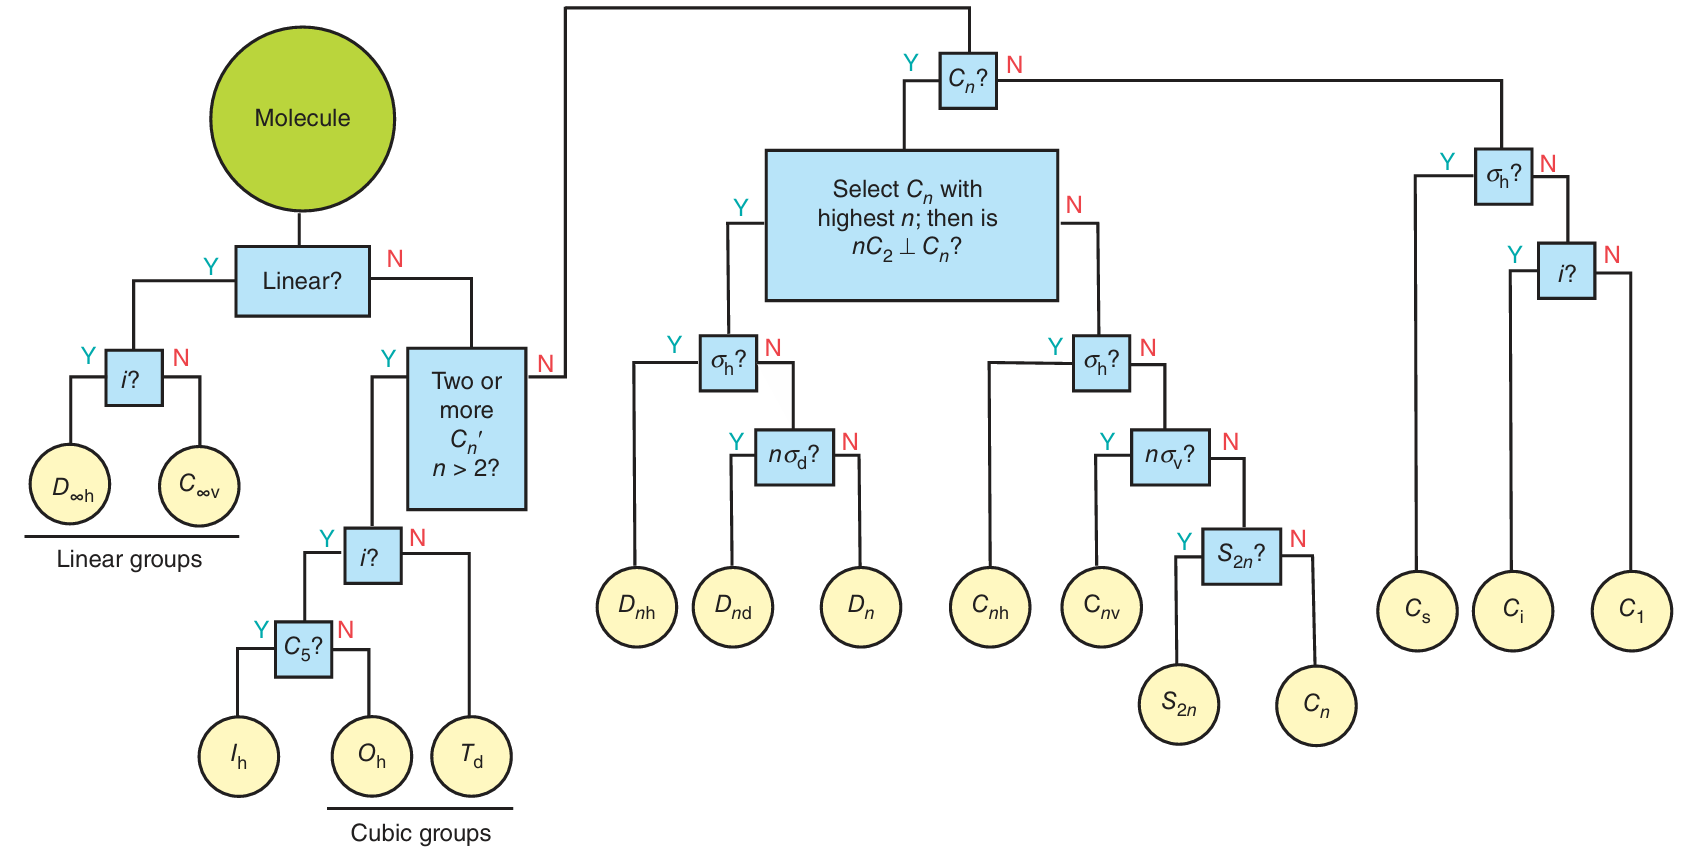
\includegraphics[scale=0.27]{Ch7/classification_sym}
			\caption{A brief flow chart for determining point groups}
		\end{figure}
			
	\subsection{Mulliken's Notation for Irreps}
		
			A represents a one-dimensional irrep that is unchanged under $C_n$ rotation.\\
			B represents a one-dimentional irrep that is antisymmetrical under $C_n$.\\
			E, T, G, H represent 2- to 5-dimensional irreps respectively.\\\ \\
			%
			Prime ' means symmetry under $\sigma_h$ while double prime '' shows antisymmetry.\\
			Subscripts g (even, gerade) and u (odd, ungerade) denotes symmetry and antisymmetry under $i$ respectively.\\
			For one-dimensional irreps, subscript 1 and 2 denotes symmetry and antisymmetry under $C_2$ or $\sigma_v$ respectively.\\\ \\
			%
			In $D_{\infty h}$ and $C_{\infty v}$ groups, 
			$\Sigma^{\pm}$ is one-dimensional with $\pm$ denoting symmetry and antisymmetry under $C_2$ or $\sigma_v$ respectively, 
			while $\Phi, \Pi, \Delta$ corresponds to two-dimensional irreps.
			
\section{Group Theory in Spectroscopy}

	\subsection{Determining Non-zero Integrals}
	
		This is the most important and fundamental use of group theory in chemistry.\\\ \\
		%
		The result of an integral does not vary with space transforms, and the differential $\text{d}x$ is independent of space. 
		Therefore for an integral to be non-zero, its integrand must contain the component of total symmetry. \\
		That is, the direct sum decomposition of the integrand's representation must \emph{contain the irrep of total symmetry}, 
		which is, under most cases $A_{1(g)}$.\\
		However, for the direct product of two irreps, \emph{only if they're the same can it contain total symmetry}.	
		Hence if the integrand is in a form of product, the factors must share at least one common irrep in their decomposition.\label{8.3.1}

	\subsection{Normal Vibration Modes}
	
		For a molecule consists of $N$ atoms it possesses in all $3N$ degrees of freedom containing 
		3 translations, 3 rotations and other $3N-6$ vibrations.
		If it's linear, there's only 2 degrees of rotation freedom and so $3N-5$ vibrations.\\\ \\
		%
		Therefore, to determine the irrep for each normal mode of vibration, 
		we first derive the representation for all the freedom degrees, then subtract the translation and rotation irreps from it and decompose.\\\ \\
		%
		The representation for all the freedom degrees can be further seperated into the composite of two parts: 
		the geometry of the molecule, and the representation for the three degrees of freedom of each atom
		(usually the vectors $x, y$ and $z$ are used for simplicity).\\\ \\
		%
		The geometrical character can be derived ultilizing the principle mentioned in \ref{8.1.1}.
		While the character for freedom degrees can also be derived in the same way, the more direct results are shown here for simplicity:
		\[\chi(C_n) = 1+2\cos\frac{2\pi}{n}, \quad \chi(S_n) = -1+2\cos\frac{2\pi}{n}\]
		The character for $\sigma$ and $i$ have already been included, see \ref{8.2.1}\\\ \\
		%
		Take $NH_3$ as an example: work out its representation for all degrees of freedom in table \ref{freed}\\
		\begin{table}
		\centering
		\begin{tabular}{p{7em}|p{7em}p{7em}p{6em}p{8em}}
			\toprule
			$\ C_{3v}$ & $\ E$ & $\ 2C_3$ & $\ 3\sigma_v$ \\
			\midrule
			$\ \Gamma_{NH_3}$ & \ 4 & \ 1 & \ 2 \\
			$\ \Gamma_{xyz}$ & \ 3 & \ 0 & \ 1 \\
			\midrule
			$\ \otimes$ & \ 12 & \ 0 & \ 2 & $=3A_1+A_2+4E$\\
			\bottomrule
		
		\end{tabular}
		\caption{Character for all degrees of freedom of $\rm NH_3$}
		\label{freed}
		\end{table} \\
		
		\!\!\!\!\!\!\!\!Therefore, the normal modes are (decomposition via \ref{8.1.3})
		\[\Gamma_{vib} = \Gamma_{NH_3} \otimes \Gamma_{xyz} - \Gamma_{trans} - \Gamma_{rot} = (3A_1+A_2+4E) - (A_1+E) - (A_2+E) = 2A_1+2E\]
		
	\subsection{Selection Rules}
	
		The probability and rate of a transition is proportional to the modulo square of the \emph{transition moment} $\mathbf{\mu}_{fi}$:
		\[\mathbf{\mu}_{fi} = \langle f | \mathbf{\hat{\mu}} | i \rangle, 
		\quad \mathbf{\hat{\mu}} = -e\mathbf{\hat{r}}, \quad \mathbf{r} = \mathbf{x} + \mathbf{y} + \mathbf{z}\]
		%
		Therefore a permitted transition between the initial and final electronic and/or vibrational state 
		should contain the same irrep as of $x, y$ or $z$ in their direct product according to the principle \ref{8.3.1}. 
		This is called the \emph{symmetry selection rule}.
		
		\subsubsection{Infrared Activity}
			As for pure vibrational IR spectra, the initial ground state is always total symmetric, 
			so IR active vibrational modes must lead to a change in molecular electric dipole, i.e. contain the irrep of $x, y$ or $z$.
		
		\subsubsection{Vibrational Raman Activity}
			Similar to IR, the initial ground state is always total symmetric too, but the operator is now $\hat{\mu}^2$ 
			which now requires the active vibrational modes to lead to a change in molecular electric dipole tensor, 
			i.e. contain the irrep of $x^2$, $y^2$, $z^2$, $xy$, $yz$ and $xz$.
			
		\subsubsection{Electronic Spectra Selection Rules}\label{laporte}
			Apart from the previous symmetry selection rule, for a central-symmetric molecule, 
			all of $x, y$ and $z$ are $u$ hence $\Gamma_f \otimes \Gamma_i = u$, 
			which implies that only $u \leftrightarrow g$ transitions are allowed. This is the \emph{Laporte selection rule}.\\\ \\
			%
			However these selection rules, for electronic spectra, aren't absolute, as vibration can distort the molecule and make symmetries vanish.
			In mathematical perspective, the electronic state and vibrational state are coupled (that's why I said `and' previously) so that
			\[\Gamma_{f,e}\Gamma_{f,vib} \otimes \Gamma_{i,e}\Gamma_{i,vib} = \Gamma_{TS} \oplus \cdots\]
			can make a non-zero transition. Where $\Gamma_{i,vib}$ is usually always $\Gamma_{TS}$.
			
	\section{Symmetry Adapted Linear Combination}\label{salc}
	
		If two orbitals can overlap and form a bond, the integral $\langle \alpha | \hat{H} | \beta \rangle$ must be non-zero, 
		and as $\hat{H}$ is total symmetrical, the symmetry of $\beta$ must match that of $\alpha$, 
		so called \emph{Symmetry Adapted Linear Combination} (SALC). \\ \\
		However orbitals that share some symmetry elements but not identical in symmetry (e.g. both A irrep or both $g$ symmetry) 
		can also interact to some extent.\\\ \\
		%	
		For a molecule with central atom and ligands, we can either rearrange the orbitals of ligands so as to match the orbitals of the central atom, 
		or rearrange the orbitals of the central atom to point towards the ligands (the latter gets the name \emph{hybridization}.\\\ \\
		%
		The following equation gives the method of \emph{projection operator} to generate the unnormalized orbital of required symmetry from a given set of basis orbitals:
		\[\boxed{| m \rangle = \sum_{R}^{\ }\chi_{m}(R)\,R|\alpha\rangle}\]
		If the orbitals generated are linearly dependent such as 3 orbitals generated for a symmetry with double degeneracy, 
		subtract to cancel the dependency.\\\ \\
		%
		After generating the adequate orbitals, all $n$ orbitals with the same symmetry mix together to give $n$ molecular orbitals, 
		and electrons fill in from the orbitals lower in energy to the ones higher.\\ \\
		For a more quantitive energy result, one can still think that 
		overlapping orbitals with the same symmetry and similar energies are prioritized (see also \ref{closer energy}), 
		and after the combination, the results can then further recombine to maximize bonding overlap and give the ultimate orbitals.\\ \\
		%
		Also it's no difference whether you rearrange the ligands or the central atom because they are the same: 
		in real molecules the process isn't done by a clear series of steps, 
		they're simultaneous and every theory that can describe how it can achieve the lowest energy state is somehow reasonable.\\\ \\  
		%
		But, hybridization in single atoms do not occur as the atomic orbitals themselves are not the same symmetry species 
		(so as the combination of ligands). 
		They do so in molecules simply because the driving force towards better overlap and lowering overall energy.
		
		\subsection{$sp$ mixing}
		It is worth noticing that as orbitals with similar energies interact better, 
		and the energy difference between different subshells within the same shell increase with the increase of principal quantum number,
		a special phenomenon occurrs in period 2 diatomic bonds known as $sp$ mixing 
		where the $s\sigma$ antibonding orbital interact with the $p\sigma$ bonding orbital, 
		leading to the elevation of $p\sigma$ bonding orbital over $p\pi$ orbitals.
		Figure \ref{spmix} illustrates this process.\\
		\begin{figure}[h]
		\centering
		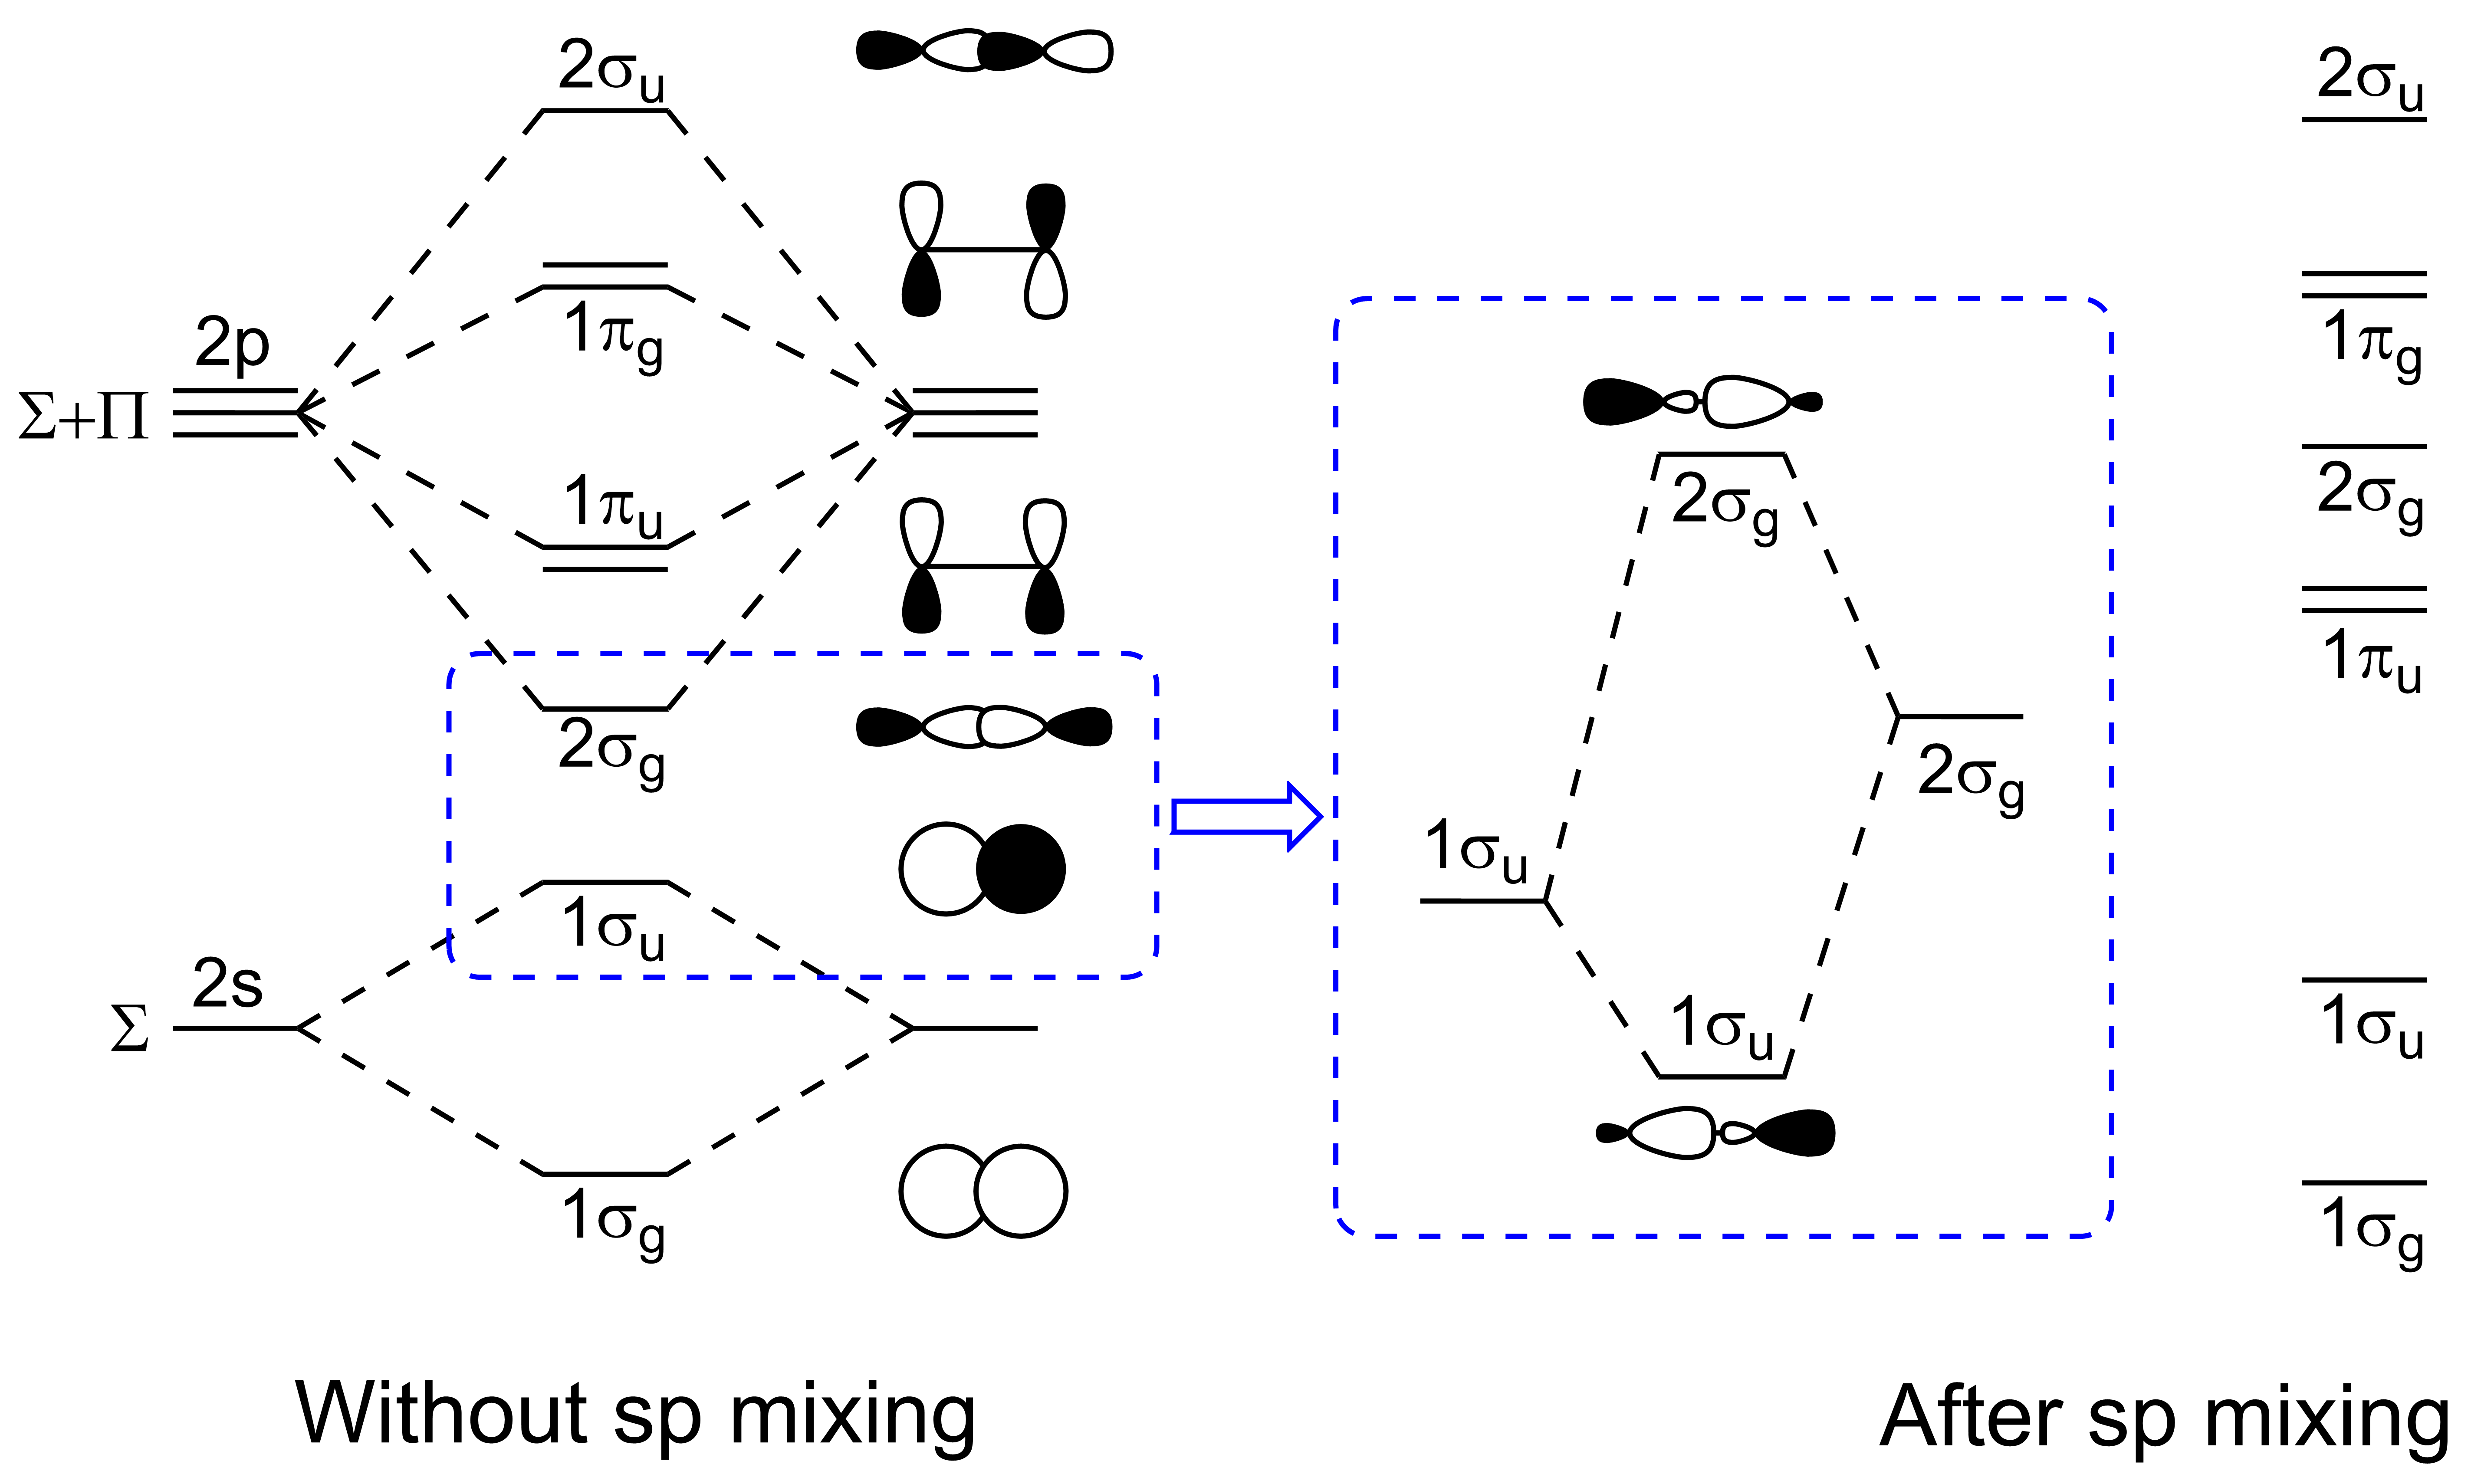
\includegraphics[scale=0.06]{Ch7/spmixing}
		\caption{$sp$ mixing in period 2 homonuclear diatomic molecules}
		\label{spmix}
		\end{figure}\\
		This effect requires close $sp$ energy level ($\approx$ 16 eV) and the limit point is somewhere near nitrogen monoxide NO.
		Figure \ref{p2trend} illustrates this trend.
		\begin{figure}[h]
		\centering
		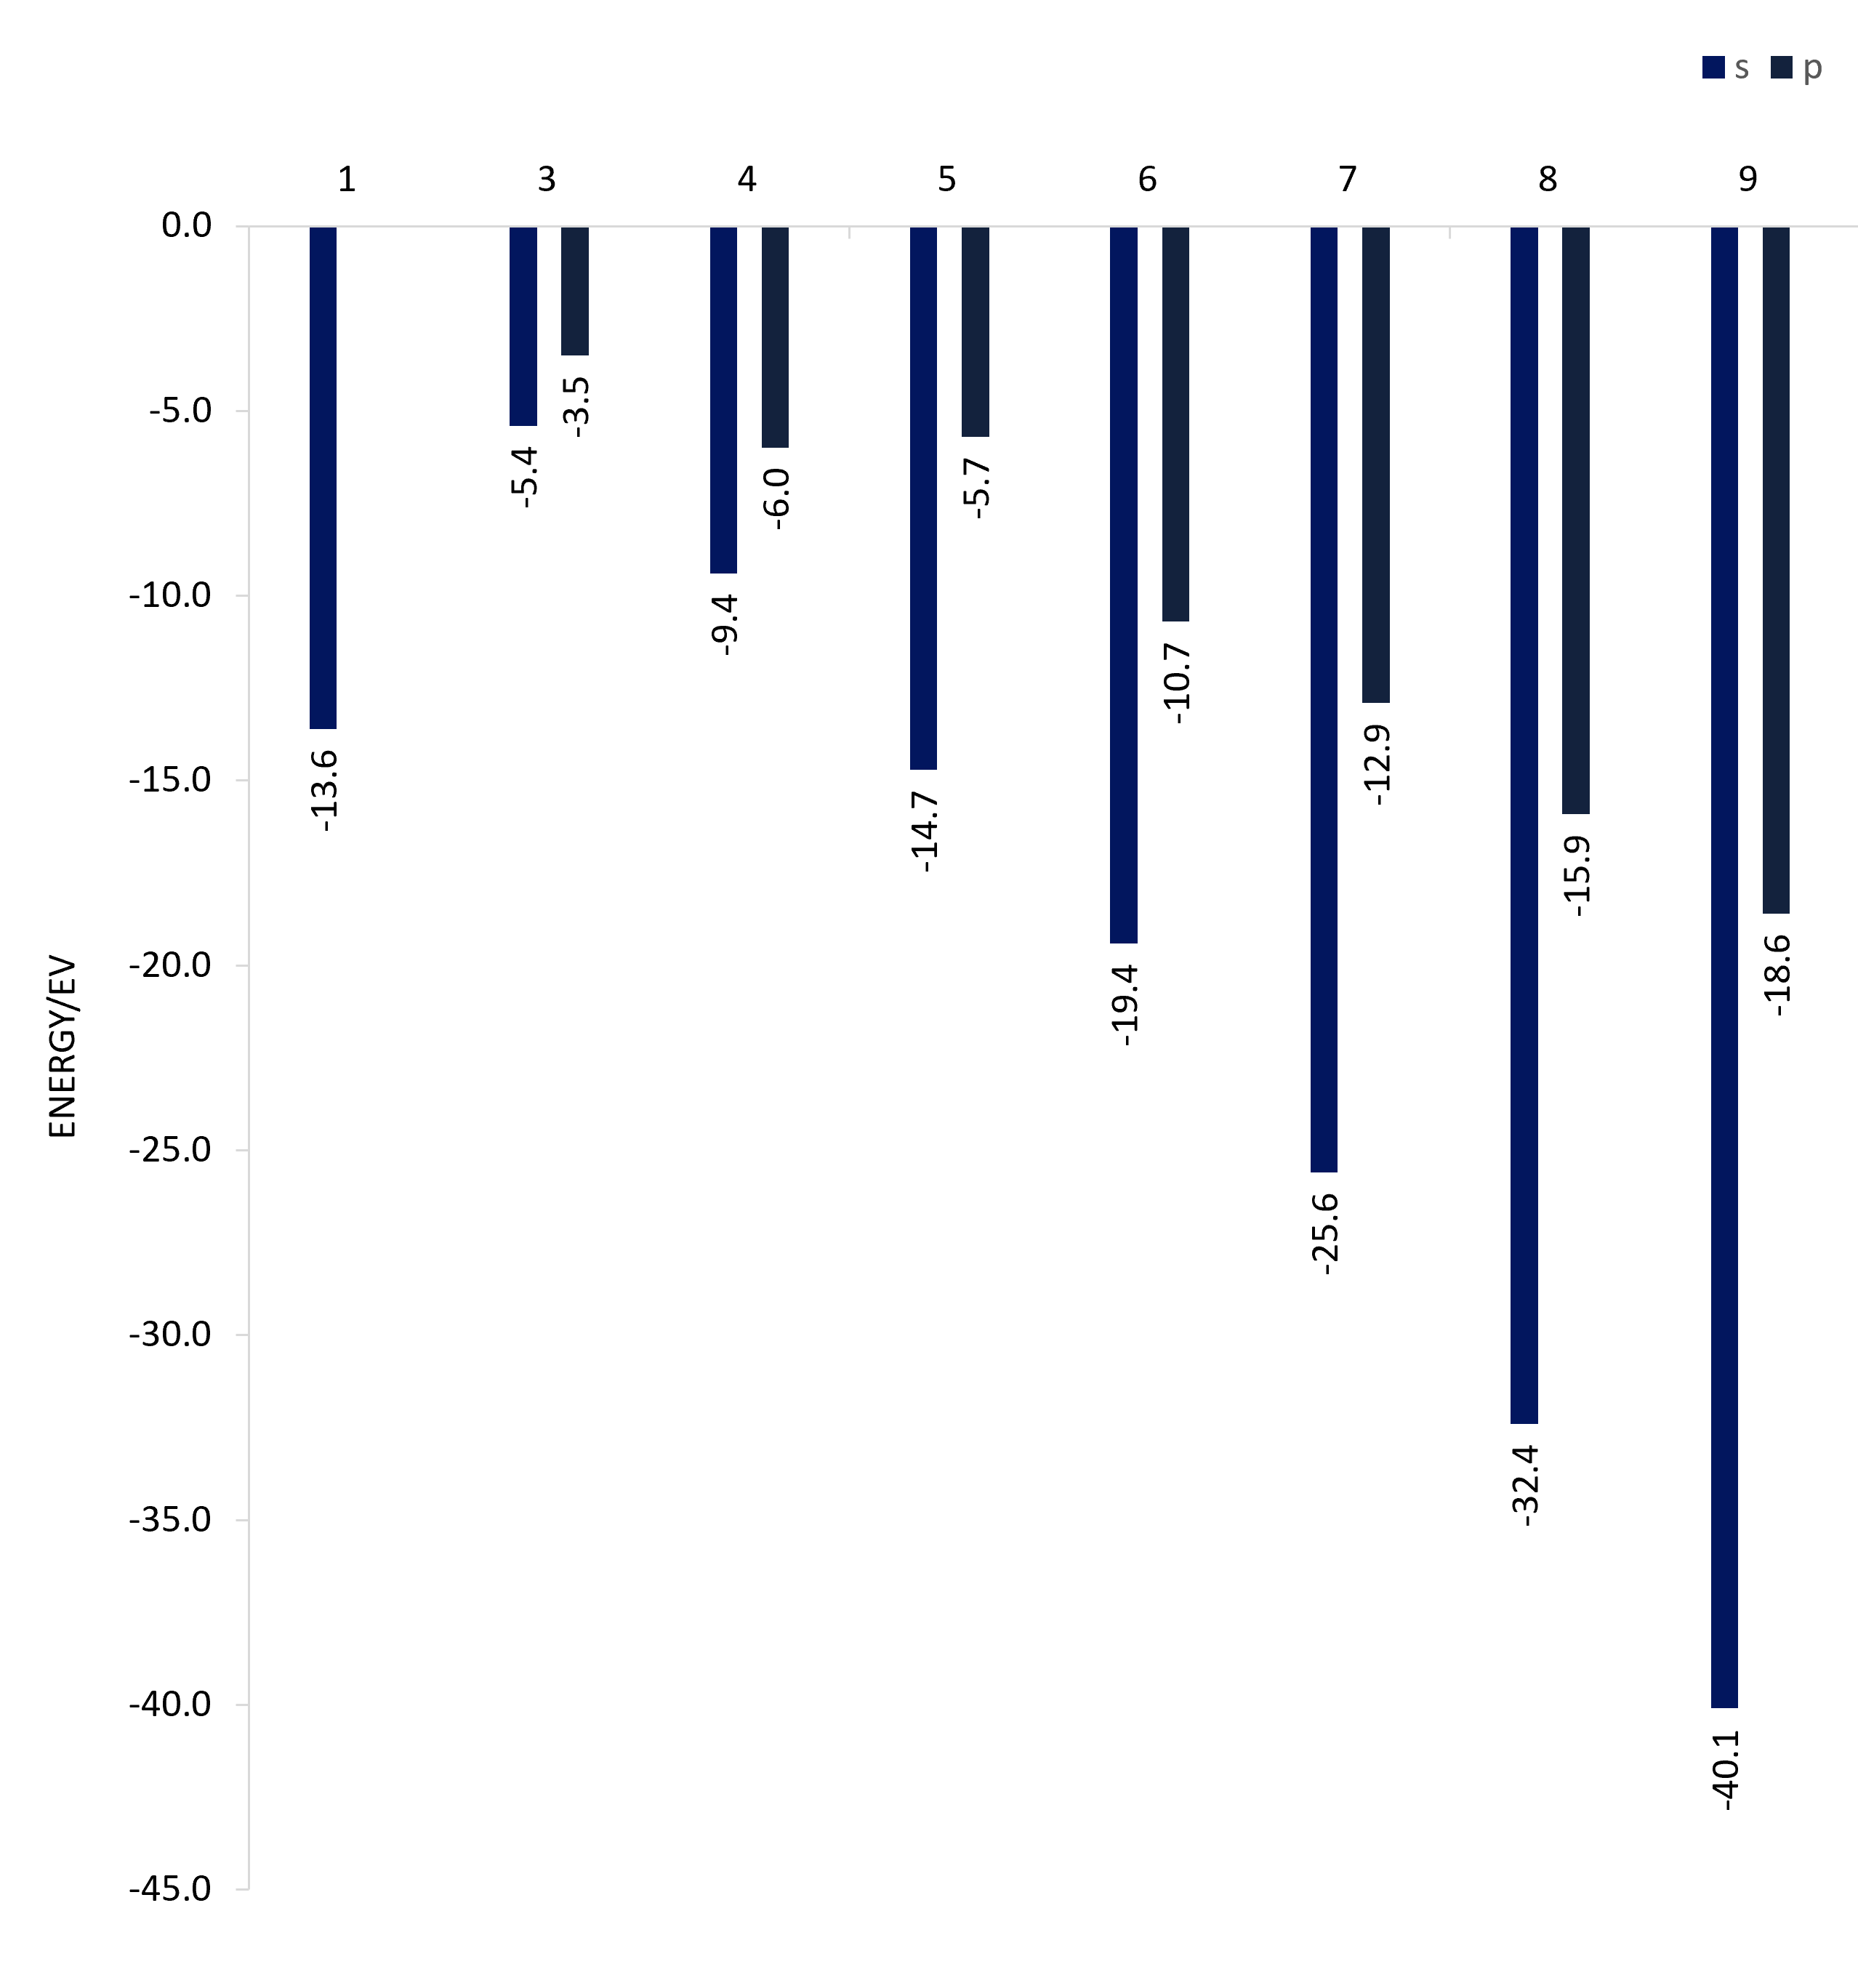
\includegraphics[scale=0.3]{Ch7/orbitale}
		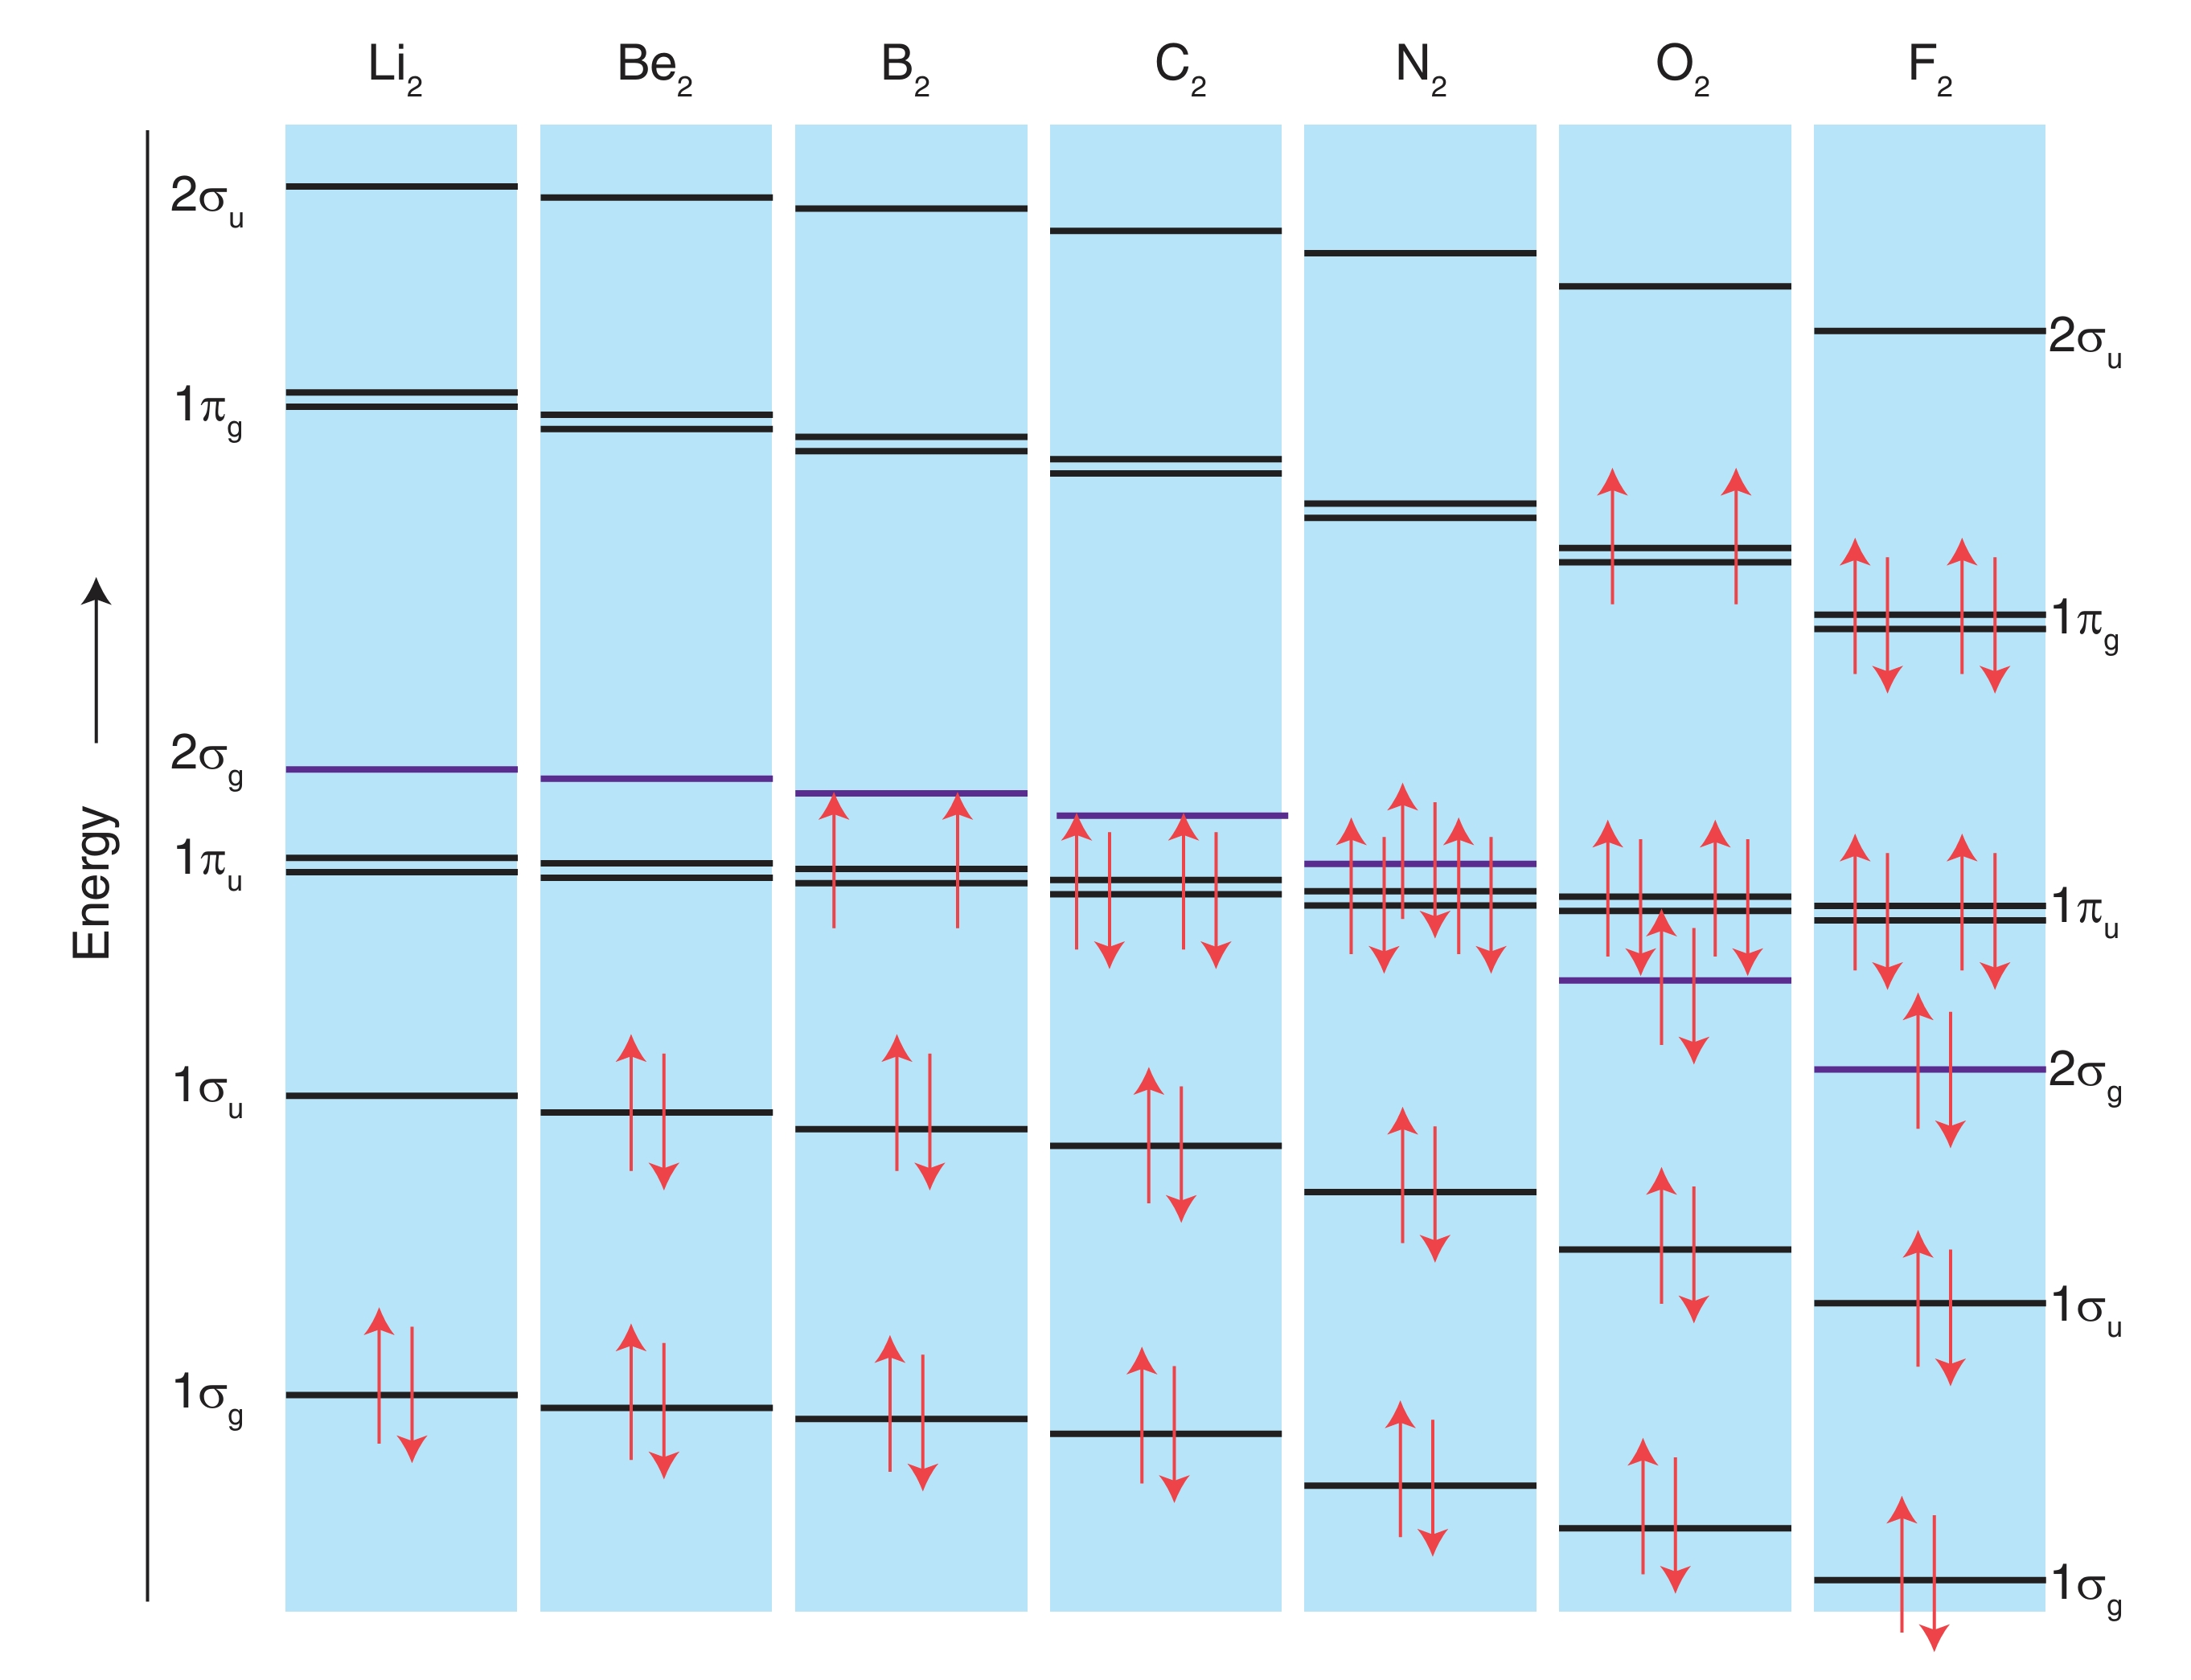
\includegraphics[scale=0.08]{Ch7/p2trend}
		\caption{AO energy and diatomic molecule orbital profile of period 2 elements}
		\label{p2trend}
		\end{figure}
		
		\subsection{Group Orbitals}
		Take $NH_3$ as an example for ligand SALC: the overall symmetry of three Hs is listed in table \ref{3h}.
		\begin{table}
		\centering
		\begin{tabular}{p{7em}|p{7em}p{7em}p{7em}p{8em}}
			\toprule
			$\ C_{3v}$ & $\ E$ & $\ 2C_3$ & $\ 3\sigma_v$ \\
			\midrule
			$\ \Gamma_{3H}$ & \ 3 & \ 0 & \ 1 & $=A_1 + E$\\
			\bottomrule
			
		\end{tabular}
		\caption{Character of $\rm NH_3$'s 3Hs}
		\label{3h}
		\end{table}\\\ \\
		%
		And the operation effect, i.e. the $R|\alpha\rangle$ term is listed in table \ref{ra}\\
		\begin{table}
		\centering
		\begin{tabular}{p{5em}|*{6}{p{5em}}}
			\toprule
			$\ C_{3v}$ & $\ E$ & $\ C_3^+$ & $\ C_3^-$ & $\ \sigma_v$ & $\ \sigma_v'$ & $\ \sigma_v''$ \\
			\midrule
			\ 1&\ 1&\ 2&\ 3&\ 1&\ 2&\ 3 \\
			\ 2&\ 2&\ 3&\ 1&\ 3&\ 1&\ 2 \\
			\ 3&\ 3&\ 1&\ 2&\ 2&\ 3&\ 1 \\
			\bottomrule
		\end{tabular}
		\caption{Effect of group $C_{3v}$ on $\rm NH_3$'s 3Hs}
		\label{ra}
		\end{table}\\
		%
		Therefore, the E orbitals are:
		\[|E_1\rangle = \mathbf{E} \cdot C_{3v}|1\rangle = (2,-1,-1,0,0,0) \cdot (1,2,3,1,2,3) = 2|1\rangle - |2\rangle - |3\rangle\]
		Similarly, we get two other E orbitals, which we find greater than the degenerecy, hence subtract:
		\[|E_2\rangle = |2\rangle - |3\rangle\]
		So now we can do the symmetry adapted combination as the graph shown here:
		\begin{figure}[h]
			\centering
			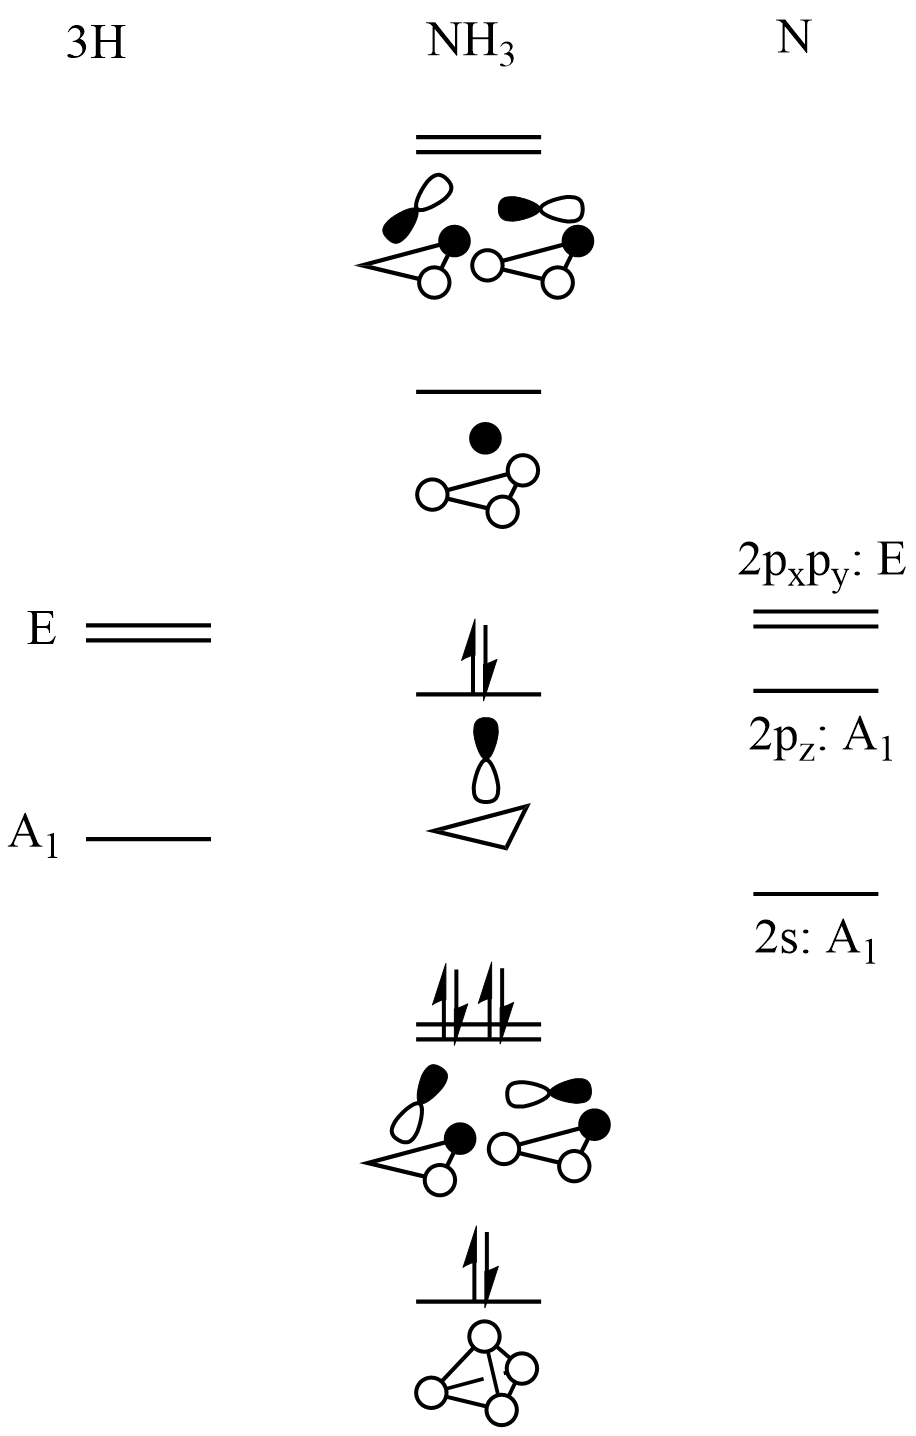
\includegraphics[scale=0.2]{Ch7/NH31}
			\qquad\qquad
			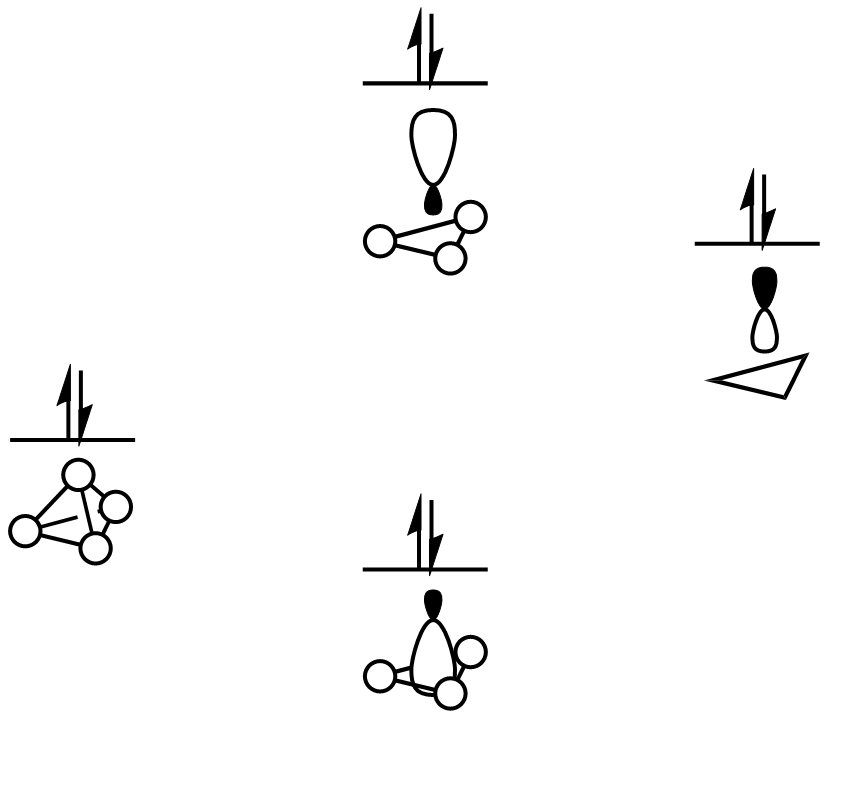
\includegraphics[scale=0.2]{Ch7/NH32}
			\caption{The orbital energy profile of $NH_3$ after first combination of symmetry adapted ligand orbitals}
			\caption{The second combination of two previous MOs, leading to the elevation of the non-bonding lone pair}
		\end{figure}\\
		Note that we actually generated the MOs of $H_3$ molecule and then match it with the AOs of nitrogen, which means this method can also generate molecular orbitals. \label{mo}
		
		\subsection{Hybridization Example}\label{hybridization}
		Take $CH_4$ as an example for central atom hybridization: 
		derive the required character for the orbitals pointing towards the vertices of a tetrahedron as in table \ref{ch4}\\
		\begin{table}
		\centering
		\begin{tabular}{p{5em}|*{6}{p{5em}}}
			\toprule
			$\ T_d$ & $\ E$ & $\ 8C_3$ & $\ 3C_2$ & $\ 6S_4$ & $\ 6\sigma_d$\\
			\midrule
			$\ \Gamma$ &\ 4&\ 1&\ 0&\ 0&\ 2&\ $=A_1+T_2$\\
			\bottomrule
		\end{tabular}
		\caption{Character for tetrahedral symmetry}
		\label{ch4}
		\end{table}\\\ 
		%
		Therefore the choice of orbitals can be the $A_1$ of $s$ and the $T_2$ set of $p_x, p_y, p_z$ or $d_{xy}, d_{xz}, d_{yz}$, 
		which corresponds to $sp^3$ and $sd^3$ hybridization.
		
	\section{Molecular Term Symbols}\label{molecular term}
	\subsection{When Electronic Configuration Dominates}
	
	When the gap between energy levels are sufficiently larger than electron pairing, 
	the state will split and give spectral terms in the same configuration but different in spin multiplicity and angular momentum.\\\ \\
	%
	Consider the simpliest case of an open-shell MO occupied by 2 electrons. Their state is the direct product of each one's state space.
	And the effect of group element on it is $RV \otimes RV = (R\otimes R)(V\otimes V)$.\\\ \\
	%
	This composite state can be decomposed into the direct sum of the orthonormal 
	\emph{symmetrical subspace} $V_+$ and \emph{antisymmetrical subspace} $V_-$. 
	Any composite state can be decomposed into symmetrical and antisymmetrical subspace components as denoted:
	\[|i\rangle \otimes |j\rangle = |ij\rangle = |ij_+\rangle \oplus |ij_-\rangle\]
	These two components are eigenvectors with eigenvalues $\pm1$ of the exchange operator $\hat{S}$, 
	and as they are orthonormal, the projection operators onto the subspaces possess these properties:
	\[\hat{S}|ij_\pm\rangle = \pm|ij_\pm\rangle, \quad \hat{P}_\pm|ij_\pm\rangle = |ij_\pm\rangle, \quad \hat{P}_\pm|ij_\mp\rangle = 0\]
	Therefore the projection operators can be consturcted by $I$ and $\hat{S}$, 
	and the effect of the group elements on the subspaces would be:
	\[R_\pm = \hat{P}_\pm(R\otimes R) \text{\ \ where\ \ } \hat{P}_\pm = \frac{1}{2}(I \pm \hat{S})\]
	And hence the character is:
	\[\chi_\pm(R) = \Tr\, \hat{P}_\pm(R\otimes R) = \frac{1}{2}\left( \Tr\, R\otimes R \pm \Tr\, \hat{S}(R\otimes R)\right)\]
	While the first term is $\chi^2(R)$, the second term must be carried out explicitly:
	\[\begin{aligned}
		\Tr\ \hat{S}(R\otimes R) & =\sum_{ij}\left\langle ij \left| \hat{S}(R\otimes R) \right| ij \right\rangle
		= \sum_{ij}\left\langle ij \left| (R\otimes R) \right| ji \right\rangle \\
		& = \sum_{ij}\left\langle i \left| R \right| j \right\rangle\left\langle j \left| R \right| i \right\rangle
		=\sum_{ij}R_{ij}R_{ji} = \Tr\, R^2 = \chi(R^2)
	\end{aligned}\]
	%
	Hence, for a two-electron state, the character is give by:
	\[\boxed{\chi_{\pm} = \frac{1}{2}\left(\chi^2{R} \pm \chi(R^2)\right)}\]
	Where if it's singlet, the antisymmetrical spin state, the spacial state shouls be symmetrical so take the positive sign, 
	and triplet negative vice versa.\\\ \\
	%
	Similarly for 3 and 4 electrons, see \\\emph{Advanced Structural Inorganic Chemistry} Page 146 (166).\\
	
	\subsubsection{Trends In Molecular Term Symbols}
	For an $n$-fold degenerate orbital, configurations with $k$ and $2n-k$ electrons have same term symbols but are in inversed order.\\
	For an empty or full orbital, its term symbol is $^1\Gamma_{TS}$.\\
	For a singly occupied orbital, its term symbol is $^2\Gamma$ with irrep the same as its molecular orbital.\\
	For orbitals of different irreps, the term symbols can be decomposed through direct product.\\\ \\
	%
	Take configuration $t_{2g}^2e_g^1$ in $O_h$ group as an example:
	\[\begin{aligned}
	\chi_{T+} &= (6,0,2,0,2,6,0,0,2,2) = A_{1g} + E_{g} + T_{2g}\\
	\chi_{T-} &= (3,0,-1,1,-1,3,1,0,-1,-1) = T_{1g}
	\end{aligned}\]
	Hence the term symbols are singlet $^1A_{1g}, ^1E_{g}, ^1T_{2g}$ and triplet $^3T_{1g}$.\\
	Then couple them with $e_g^1$ whose term is $^2E_g$:
	\[\text{eg } ^3T_{1g} \text{ and } ^2E_g:\  T_{1g} \otimes E_g = T_{1g} \oplus T_{2g}, 
	\ |1\rangle \otimes |\frac{1}{2}\rangle = |\frac{1}{2}\rangle + |\frac{3}{2}\rangle\]
	Which is $^4T_{1g}$ and $^4T_{2g}$ (with the largest multiplicity).
	
	\subsection{When Angular Momentum Dominates}\label{double group}
	When the gap between different energy levels is smaller than that of spin pairing, 
	and spin-orbit coupling is sufficiently small to be neglected, 
	the terms are determined by the splitting of angular momentum state $|L,m\rangle$.\\\ \\
	%
	The operation of rotating $\alpha$ radians under the basis of angular momentum is:
	\[\hat{R}(\alpha) = \exp(-\frac{i}{\hbar}\alpha\hat{L}_z)\]
	As $|L,m\rangle$ is the eigenstate of $\hat{L}_z$, it is also the eigenstate of $\hat{R}(\alpha)$, the eigenvalues are:
	\[\hat{L}_z|L,m\rangle = \hbar m|L,m\rangle\ \Rightarrow \ \hat{R}(\alpha)|L,m\rangle = \exp(im\alpha)|L,m\rangle\]
	Hence $\hat{R}(\alpha)$ is a diagonal matrix under this basis and its trace is the sum of eigenvalues:
	\[\chi(\alpha) = \sum_{m=-L}^{L}\exp(im\alpha) = \frac{e^{-iL\alpha}(1-e^{i(2L+1)\alpha})}{1-e^{i\alpha}}\]
	Invoking Euler's identity and simplify it into trig functions:
	\[\chi(\alpha) = \frac{e^{-i(L+1/2)\alpha}-e^{i(L+1/2)\alpha}}{e^{-i\alpha/2}-e^{i\alpha/2}} = \frac{\sin (L+1/2)\alpha}{\sin\alpha/2}\]
	Therefore, knowing the character, we can decompose it into direct sums:
	\[\boxed{\chi(\alpha) = \frac{\sin (L+1/2)\alpha}{\sin\alpha/2}}\]
	
	\subsection{When Spin-Orbit Coupling Dominates}
	Now the terms are determined by total angular momentum number $J$. 
	When $J$ is an integer, the formula for $L$ still holds for $J$, but when it's a half-integer, it does not, 
	because rotation of $2\pi$ is no longer an identity operation:
	\[\chi(\alpha+2\pi) = \frac{\sin (J+1/2)(\alpha+2\pi)}{\sin\alpha/2+\pi} = \frac{\sin 2\pi + (J+1/2)\alpha}{\sin\alpha/2+\pi}\]
	As $J$ is a half integer, it becomes:
	\[\chi(\alpha+2\pi) = \frac{\sin (J+1/2)\alpha}{-\sin\alpha/2} = -\chi(\alpha)\]
	Hence we multiply each of the group elements with operation $R$, rotation $2\pi$ and expand the original group, which is called \emph{double group},
	and use this to derive characters and irrep decompositions, so as to achieve the term symbol when spin-orbital coupling dominates.\\\ \\
	%
	Note that the character of $R$ when $J$ is half-integer will use L'Hopital's rule, example taken $J=1/2$:
	\[\chi(2\pi) =\lim_{\alpha \to 2\pi}\frac{\sin(1/2+1/2)\alpha}{\sin\alpha/2} = \lim_{\alpha \to 2\pi} \frac{2\cos\alpha}{\cos\alpha/2} = -2\]\\
	%
	These splitting and term symbols will be applied to coordination chemistry in ligand field splitting 
	where strong field (configuration dominates) and weak field (angular momentum dominates) have different splitting patterns. See \ref{split}\label{socouple}.
	\begin{figure}[h]
	\centering
	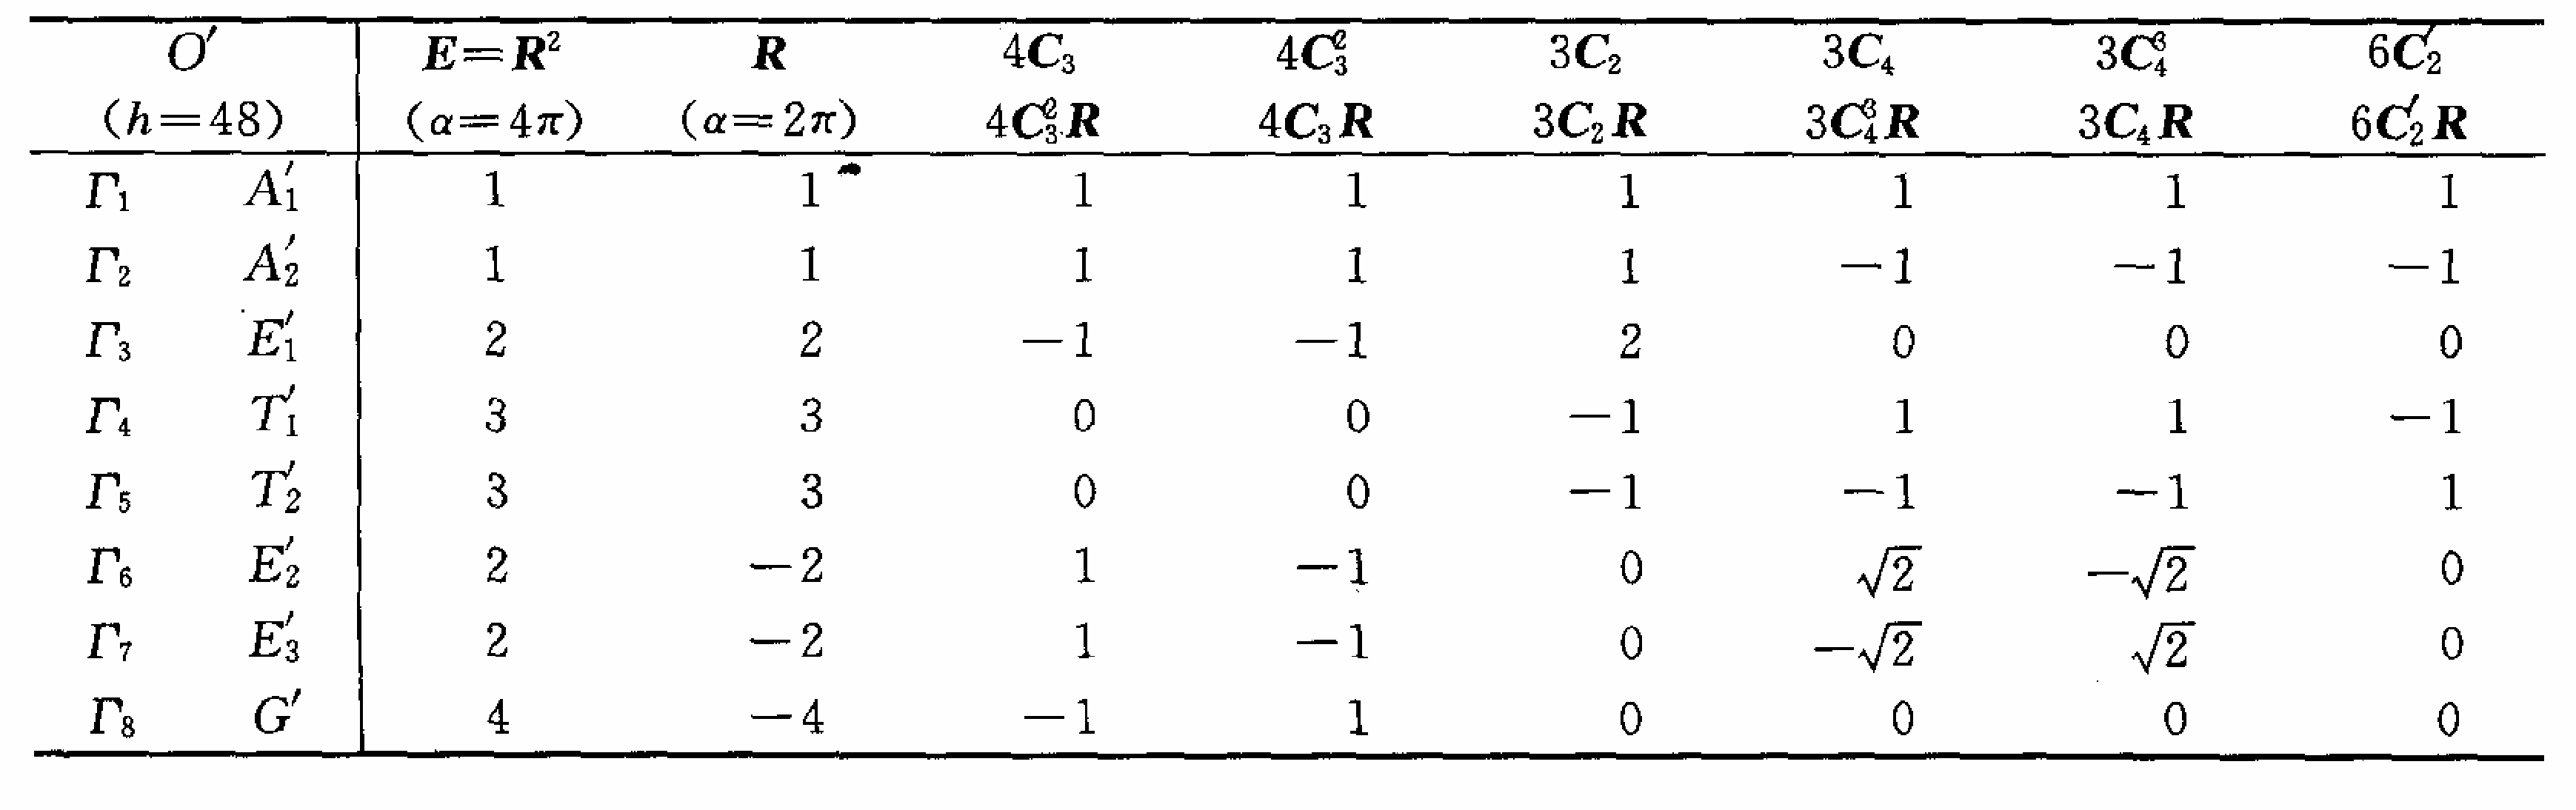
\includegraphics[scale=0.1]{Ch7/doublegroup}
	\caption{Character Table of $O_h$ Double Group}
	\end{figure}
	
	
		
		
	
	
















